\chapter{Details about the Brine-Water heat pump test-rig}
\label[secinapp]{chap:bwp-components}
\resetallacronyms

\section{History}
\label[secinapp]{sec:bwp-history}

The \BWP{} has being designed at the beginning of the thesis work, in
2009. It has been built between 2009 and 2010, and has been used to
test compression units prototypes in 2010, 2011, and in
2013\footnotep{See \cpref{sec:potential-demo} for details about the
  timeline of the experimental setups in the project.}. In Automn
2010, the prototype has been heavily modified, as detailed in
\cref{sec:bwp-redesign-1}. It has been modified again, between Winter
2012 and Automn 2013, as detailed in \cref{sec:bwp-redesign-2}.

During the tests performed between 2010 and 2011 with the \BWP{}, the
compression units from the \textit{evo1}, the \textit{evo2}, and the
\textit{evo3} design families failed and crashed, as the units from
those design families were not ready for integration into heat pump
circuits. The units from those families that have been tested have
broken soon after the beginning of the tests because of design,
manufacturing, balancing, or internal set up problems. Compression
units from \textit{evo3} have been tested in the \BWP{} but failed to
provide stable data or failed to develop pressure ratios or rotor
speeds high enough to produce valuable datasets. Compression units
from \textit{evo3} were also breaking soon after the beginning of the
test campaigns. The units from those 3 families failed before the
production of any valuable datasets or stable \OP{}. They had been
tested first in a gas loop at the industrial partner facility, but
most of the issues could only reveal themselves at production rotation
speeds\footnotep{The compression units rotational speed in the
  industrial partner gas loops was limited due to technical
  limitations.} and in real heat pump conditions. The compression unit
mounted in the \BWP{} for the experiment which has been used to
generate the data presented in \cref{sec:bwp-perfs} was the
\textit{cp101} unit, from the \textit{evo4} design
family\footnotep{Details about the previous design families are given
  in \cpref{sec:bwp-history}.}. This unit had been used successfully
in a Brine/Water heat pump test-rig at a research center of the
industrial partner and had been replaced there by a compression unit
from the \textit{evo5} design family\footnotep{The \textit{evo5}
  design family was focused on improving the compression unit
  performance, which was below the models predictions due to different
  identified issues.}. The unit had been partially dismantled,
checked, and cleaned up before being delivered to be mounted in the
\BWP{}\footnotep{The front part, with volutes, impellers, and shaft,
  had been dismantled and mounted again. The motor cooling area had
  not been checked or dismantled.}. Unfortunately the unit tested in
the \BWP{} in 2013, \textit{cp101}, crashed soon after the beginning
of the experiment. Before the crash of the unit, a small B8.0/W11.0
was being stabilized, with the compressors being connected in series,
being bypassed with the new bypass system. The data collected during
that experiment and their interpretation are presented in
\cref{sec:bwp-perfs}. After the crash, the compression unit has been
dismantled for analysis at the industrial partner research center. It
turned out that one of the volute parts at the second compression
stage had not been screwed back well in place during the maintenance
operations performed before the delivery to EPFL. When the temperature
rose in the circuits and in the compression unit, during the
experiment, the thermal expansion phenomena have released the part,
which has moved slightly, with the forces applied by the \BWP{} pipes
and circuits\footnotep{The compression units mounting is hyperstatic
  due to the number of pipes and directions for the connections. This
  hyperstatism creates forces when the pipes are plugged in. Moreover,
  the dilatation processes also influence the forces on the different
  parts.}. Consequently, the second stage impeller touched the volute,
and a part of the labyrinth seal started to touch the impeller
surface. The shaft being unbalanced by the increasing touching forces
touched the set of radial bearings. The shaft broke between the radial
and the set of axial bearings, due to the too big torsion forces in
the shaft, and welded together with the set of radial bearings, due to
the energy released by the touching.

\subsection{First set of heavy modifications}
\label[secinapp]{sec:bwp-redesign-1}

The first set of heavy modifications was dedicated to the solving of
topology issues related to weight measurements. In order to measure
the weight of the heat exchangers and of the economizer, those
components were connected to the main circuits using flexible
pipes. In the very first version of the experimental setup, the
flexible pipes were bent. When bent, the rigidity of the flexible
pipes is a function notably of the pressure inside the pipe. As the
pressure changes, the efforts on the flexible pipes change, which
influences the value measured by the load cells. Additionally, as the
flexible pipes were changing the efforts together, they were creating
an hysteresis effect which could not be compensated with simple
calibration processes.

\subsection{Second set of heavy modifications}
\label[secinapp]{sec:bwp-redesign-2}

The second set of heavy modifications was dedicated to the adaptation
of the \BWP{} to the layout of the compression units of the
\textit{evo4} design family. Indeed, the \BWP{} initial version had
been designed with the inlets and outlets locations of the previous
generations, \textit{evo 1 to 3}. Those locations have changed between
\textit{evo3} and \textit{evo4} because the industrial partner,
responsible of the design and production of the devices, has
redesigned the shapes and size of the volute parts. With the re-design
specifications and needs, it was not possible to keep the same
location for the inlets and outlets. The design of the flanges have
also changed between \textit{evo3} and \textit{evo4}, in order for the
compression unit to be mounted on the \BWP{} or the \AWP{}
indifferently. This change of layout has implied to modify heavily the
piping of the upper part of the \BWP{}. Those piping modifications also
included the new version of the bypass circuits\footnotep{See
  \cpref{sec:bwp-bypass-system} for details about the evolution of the
  \BWP{} bypass circuits.}, of the motor cooling
circuit\footnotep{See \cpref{sec:bwp-motor-cooling} for details about
  the evolution of the \BWP{} motor cooling circuit.}, and of the gas
bearings aeration circuits\footnotep{See \cpref{sec:bwp-aeration} for
  details about the evolution of the \BWP{} gas bearings aeration
  circuit.}. Originally, those circuits design were close to the
circuits tested in the \AWP{}. Taking in account the issues
encountered with the \AWP{}, those circuits have been modified in the
\BWP{} before restarting the tests in 2013.

\section{Gas bearings aeration circuit layout and topology}
\label[secinapp]{sec:bwp-aeration-details}

The Gas bearings aeration circuit starts at the top of the
installation, at the second stage compression outlet. Physically, it
starts downstream of the beginning of the bypass circuit, before the
check valve. The beginning of the gas bearings aeration circuit is on
the bypass circuit, at its very beginning, because of space
constraints. The latter has to start very close from the main vapor
line. Indeed, as there is no flow in the bypass circuit in normal
operation, the gaseous refrigerant in this circuit may
condensate. Locating the inlet of the gas bearings aeration circuit
close to the main vapor line avoids that such condensate flows into
the aeration circuit. The gas bearing aeration circuit goes down with
a 1/2-inch pipe. The circuit is made of a manual needle valve which
allows to decrease the flow if needed\footnotep{As explained in
  \cpref{sec:awp-issue-bearings-aeration}, the flow in the gas
  bearings aeration circuit was already low, so this valve was not
  fully open during the experiments.}, and a coriolis mass flow
meter. Then, the circuit was divided into two branches of
approximately the same lengths and level of sophistication, in order
to get approximately the same level of pressure drop in the two
branches. The two branches of 1/2-inch diameter were equipped with a
0.5mm-filter able to be bypassed by the opening of a solenoid
valve. Close to the unit, the diameter of the circuits is reduced to
1/4 of inch. The two branches inject cold gas at the bottom of the
compression unit and at the top of the axial bearing. An electric
resistance coiled around the circuit pipe downstream of the mass flow
meter allows to be sure to inject superheated cold gas in the
compression unit, as no liquid droplet is allowed there. The electric
resistance is used as a security measure. The gas flow leaves the
compression unit with a significant superheat value and is injected
through a 1/2-inch pipe into the first stage separator.

\section{Motor cooling circuit layout and topology}
\label[secinapp]{sec:bwp-motor-cooling-details}

The \BWP{} motor cooling circuit starts at the bottom of the
prototype, at the condenser outlet. The circuit is made of a
co-tubular counter-flow heat exchanger\footnotep{A heat exchanger from
  the HE series, HE 1.5, from \citet{danfoss-2015c}.}  connected to a
coriolis mass flow meter. This part of the circuit is horizontal. Then
the circuit is vertical and includes a check valve located close to
the top of the installation made with 1/2-inch pipes. An expansion
valve is located at the top of the vertical pipe. The liquid
refrigerant flow is expended in the valve and the gas/liquid flow
resulting from the expansion is spread down into the motor cooling
chamber about 50 cm below, through a 1/2-inch pipe. This portion of
the circuit includes a sight glass. The motor is cooled down by the
2-phase refrigerant flow which is then collected at the evaporator
inlet through a 1/2-inch pipe.


\section{Components}
\label[secinapp]{sec:bwp-components}

\subsection{Expansion devices}
\label[secinapp]{sec:bwp-exp-devices}

\BWP{} inline components could be mounted in parallel in the prototype
housing in order to test the behavior of the cycle or of the prototype
control strategies using different type of
devices. \Cref{fig:bwp_exp_sections} shows an example of inline
components mounted in parallel with an expansion valve test
section. The 3 valves mounted in the section are a stepper motor
valve, a manual micrometer valve, and a regular thermostatic expansion
valve.

The valves that could have been tested were (sorted from the cheaper
to the more expensive):

\begin{itemize}
\item Manual micrometer valves\footnotep{Bellows-sealed metering
    valves, BM series from \citet{swagelok-valves-2015a},
    for instance.}, or capillary tubes;
\item Thermostatic expansion valves\footnotep{Thermostatic expansion
    valves, TUA series, from \citet{danfoss-tua-2015a}, for
    instance.};
\item Sporlan stepper-motor valves\footnotep{Electric expansion
    valves, SER series, from \citet{sporlan-ser-2015a}, for instance.};
\item Siemens modulating refrigerant valves with magnetic
  actuator\footnotep{Electric expansion valves for fluorinated
    refrigerants, AKV series, from \citet{danfoss-akv-2015a}, for
    instance.}.
\end{itemize}

\begin{figure}[htbp]
  \centering
  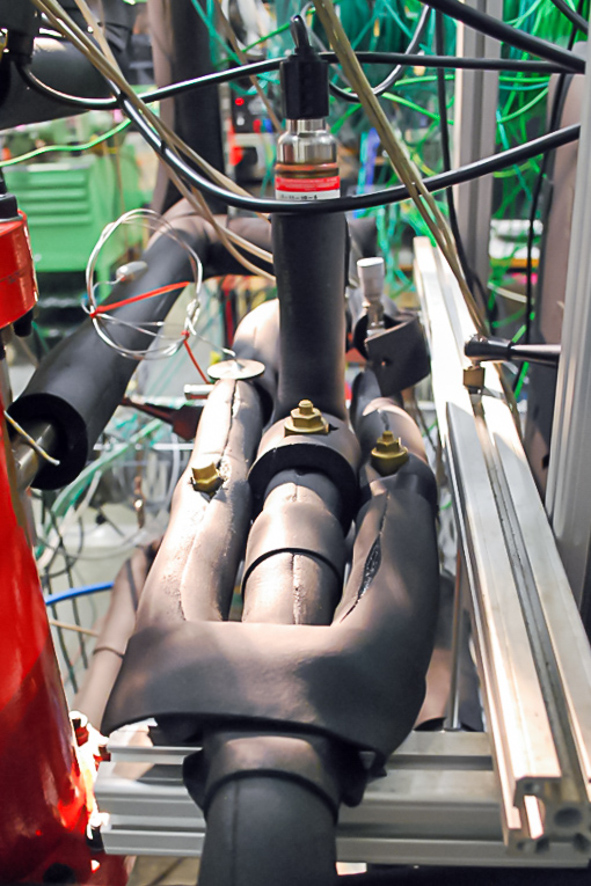
\includegraphics[width=6.6cm]{20130924T174626-3857-mod}
  \caption{BWP expansion devices section}
  \label{fig:bwp_exp_sections}
\end{figure}


\subsection{Load cells}
\label[secinapp]{sec:bwp-load-cells}

The \BWP{} is equipped with load cells to measure the weight of the
elements which are subject to variations of their overall refrigerant
vapor quality. Those weighted components are the condenser, the
evaporator, and the economizer.

These load cells were intended to be used to study the migration of
the liquid refrigerant through the circuits during the experiments and
to correlate the amount of liquid present in the different areas of
the heat pump circuits with the external heat and electric powers and
temperature conditions.

\begin{figure}[htbp]
  \centering
  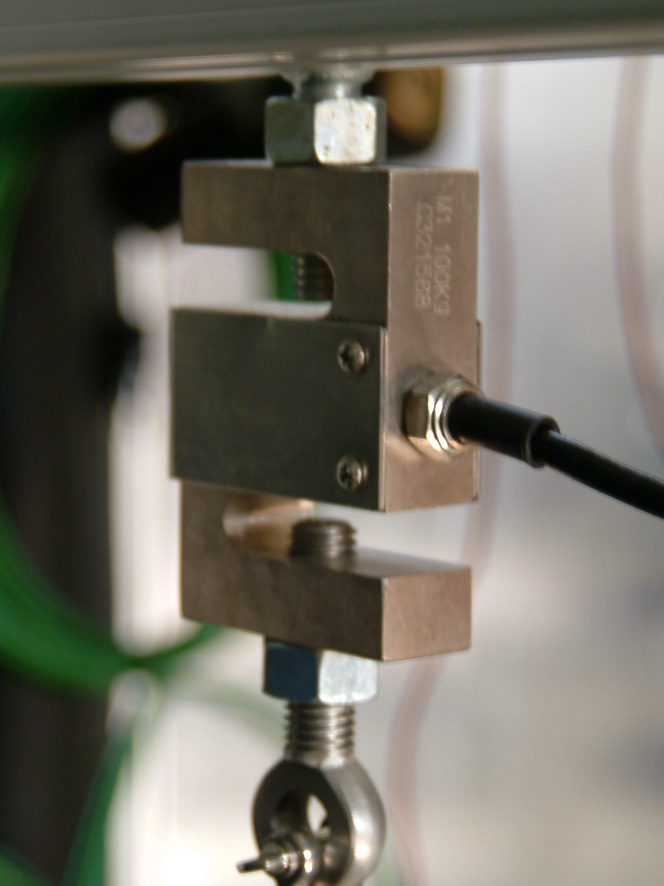
\includegraphics[width=6.6cm]{20100204-T114912-10335}
  \caption{Load cell used in the BWP}
  \label{fig:bwp-load-cell}
\end{figure}

\subsection{First stage separator}
\label[secinapp]{sec:bwp-separator}

The first stage separator is a tank able to contain a significant share
of the refrigerant charge filled in the circuits. Its role is to prevent
the suction of liquid refrigerant in the first compression stage. This
situation happens in case of a prototype control failure, as the
superheat at the evaporator outlet is too low. It this case, mist, or
even a 2-phase flow with flowing liquid, can enter the separator. This
liquid refrigerant comes in with lubricant oils\footnotep{Mineral or
synthetic lubricant oil, and dusts and particules can accumulate in the
evaporator, as detailed in \cpref{sec:awp-issue-oil+corrosion}.}, if
some are present in the evaporator.

The separator of the \BWP{} is glass-made, in order to allow an easy
monitoring of the flow characteristics at the critical location of the
circuit during the experiments. Both inlets and outlets are located at
the top of the cylinder, as it is important to be able to separate
this device to clean it up, which is far easier to do if all the
connections with the circuits are on one side. An improvement of this
design would be to add a flange at the bottom of the device, in order
to be able to open the separator for cleaning operations without
dismantling the glass part, which is particularly fragile and
vulnerable to scratches and shocks. This flange would be equipped with
a Schradder valve in order to be able to purge the separator. In the
same spirit, it is a good practice to add a Schradder valve on the
pipe at the lowest connection with the evaporator, in order to be able
to purge the lubricant oil which accumulates in the evaporator (if the
installation has been polluted, of course).

\begin{figure}[htbp]
  \centering
  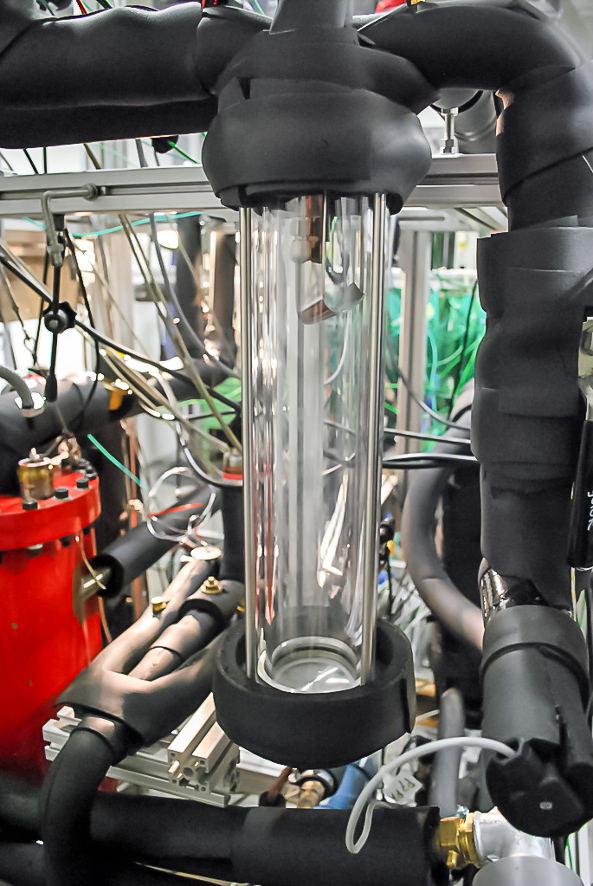
\includegraphics[width=6.6cm]{20130924T174614-3854-mod}
  \caption{First stage compressor inlet separator, in the BWP}
  \label{fig:bwp-1st-sep}
\end{figure}

The glass cylinder has a diameter of 10 cm and a thickness of 5 mm. It
would have been interesting to increase the cylinder internal
diameter, but it would have resulted in a much thicker cylinder and it
would have been quite dangerous to work with the prototype. Indeed,
the cylinder being pressurized, having glass parts is dangerous as a
defect of the glass or its damaging during a maintenance operation
could result in a glass pressure vessel explosion during an
experiment. Consequently, the diameter and the thickness need to be
kept at reasonable values.


\subsection{Economizer}
\label[secinapp]{sec:bwp-eco}

The \BWP{} economizer is not glass-made, like the \AWP{} economizer,
as it was made from a stainless steel cylinder with flanges and a
glass window which was part of a previous experimental setup. The big
size of the cylinder was an advantage and allowed safer conditions
during the experiments. Moreover, the oversizing of the parts, for the
conditions of use in the \BWP{}, was also an advantage regarding
personal security. The initial parts have been modified for the needs
of the prototype:

\begin{itemize}
\item A glass insert has been added on top of the upper flange, in
order to light the inside of the cylinder.
\item An inlet for the gas/liquid flow has been added at 2/3 of the
height of the cylinder. This inlet is oriented towards the bottom of the
cylinder with an angle of 10 degrees with the horizontal level.
\item Appropriate fittings have been fastened at the 3 inlets/outlets of
the economizer.
\end{itemize}

\begin{figure}[htbp]
  \centering \subfloat[View \#1]
  {\label{fig:bwp-eco-1}
    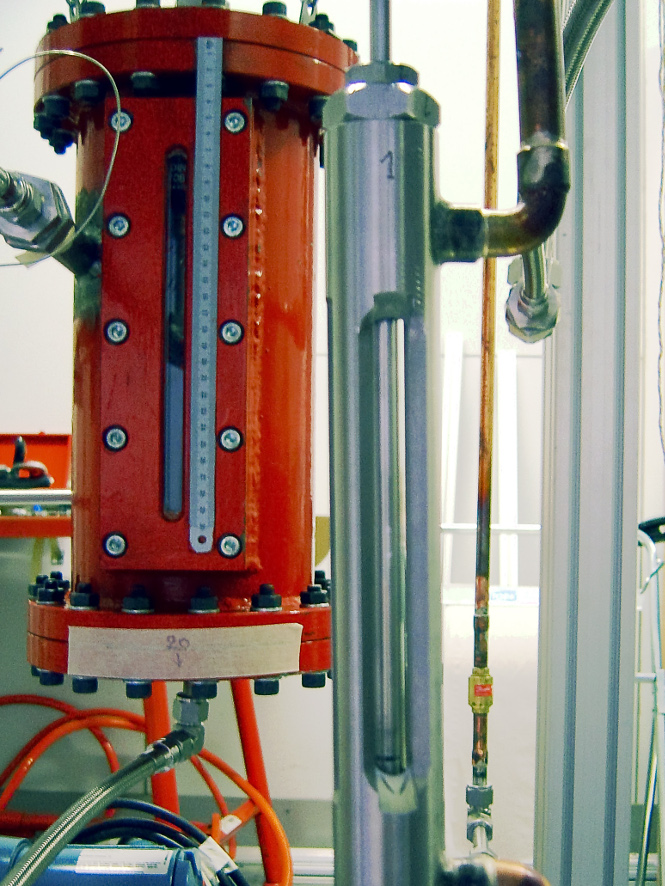
\includegraphics[height=5.5cm]{20100902-T092550-05906-mod}}
  \hspace{1em} \subfloat[View \#2]
  {\label{fig:bwp-eco-2}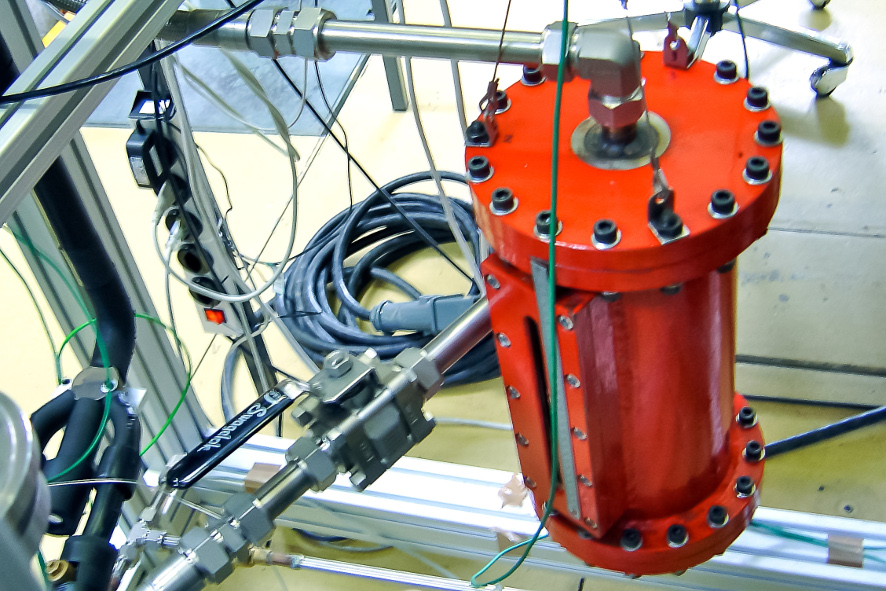
\includegraphics[height=5.5cm]{DSC00171-mod}}
  \caption{Economizer of the BWP}
  \label{fig:bwp-eco}
\end{figure}

\subsection{Pipes and fittings}
\label[secinapp]{sec:bwp-pipes}

This topic is detailed in \cpref{sec:awp-pipes}.

\bibliographystyle{plainnat}
\bibliography{main}
\label[secinapp]{sec:bwp-components-refs}
